% Options for packages loaded elsewhere
\PassOptionsToPackage{unicode}{hyperref}
\PassOptionsToPackage{hyphens}{url}
\PassOptionsToPackage{dvipsnames,svgnames,x11names}{xcolor}
%
\documentclass[
  letterpaper,
  DIV=11,
  numbers=noendperiod]{scrartcl}

\usepackage{amsmath,amssymb}
\usepackage{iftex}
\ifPDFTeX
  \usepackage[T1]{fontenc}
  \usepackage[utf8]{inputenc}
  \usepackage{textcomp} % provide euro and other symbols
\else % if luatex or xetex
  \usepackage{unicode-math}
  \defaultfontfeatures{Scale=MatchLowercase}
  \defaultfontfeatures[\rmfamily]{Ligatures=TeX,Scale=1}
\fi
\usepackage{lmodern}
\ifPDFTeX\else  
    % xetex/luatex font selection
    \setmainfont[]{Arial}
\fi
% Use upquote if available, for straight quotes in verbatim environments
\IfFileExists{upquote.sty}{\usepackage{upquote}}{}
\IfFileExists{microtype.sty}{% use microtype if available
  \usepackage[]{microtype}
  \UseMicrotypeSet[protrusion]{basicmath} % disable protrusion for tt fonts
}{}
\makeatletter
\@ifundefined{KOMAClassName}{% if non-KOMA class
  \IfFileExists{parskip.sty}{%
    \usepackage{parskip}
  }{% else
    \setlength{\parindent}{0pt}
    \setlength{\parskip}{6pt plus 2pt minus 1pt}}
}{% if KOMA class
  \KOMAoptions{parskip=half}}
\makeatother
\usepackage{xcolor}
\setlength{\emergencystretch}{3em} % prevent overfull lines
\setcounter{secnumdepth}{-\maxdimen} % remove section numbering
% Make \paragraph and \subparagraph free-standing
\makeatletter
\ifx\paragraph\undefined\else
  \let\oldparagraph\paragraph
  \renewcommand{\paragraph}{
    \@ifstar
      \xxxParagraphStar
      \xxxParagraphNoStar
  }
  \newcommand{\xxxParagraphStar}[1]{\oldparagraph*{#1}\mbox{}}
  \newcommand{\xxxParagraphNoStar}[1]{\oldparagraph{#1}\mbox{}}
\fi
\ifx\subparagraph\undefined\else
  \let\oldsubparagraph\subparagraph
  \renewcommand{\subparagraph}{
    \@ifstar
      \xxxSubParagraphStar
      \xxxSubParagraphNoStar
  }
  \newcommand{\xxxSubParagraphStar}[1]{\oldsubparagraph*{#1}\mbox{}}
  \newcommand{\xxxSubParagraphNoStar}[1]{\oldsubparagraph{#1}\mbox{}}
\fi
\makeatother


\providecommand{\tightlist}{%
  \setlength{\itemsep}{0pt}\setlength{\parskip}{0pt}}\usepackage{longtable,booktabs,array}
\usepackage{calc} % for calculating minipage widths
% Correct order of tables after \paragraph or \subparagraph
\usepackage{etoolbox}
\makeatletter
\patchcmd\longtable{\par}{\if@noskipsec\mbox{}\fi\par}{}{}
\makeatother
% Allow footnotes in longtable head/foot
\IfFileExists{footnotehyper.sty}{\usepackage{footnotehyper}}{\usepackage{footnote}}
\makesavenoteenv{longtable}
\usepackage{graphicx}
\makeatletter
\newsavebox\pandoc@box
\newcommand*\pandocbounded[1]{% scales image to fit in text height/width
  \sbox\pandoc@box{#1}%
  \Gscale@div\@tempa{\textheight}{\dimexpr\ht\pandoc@box+\dp\pandoc@box\relax}%
  \Gscale@div\@tempb{\linewidth}{\wd\pandoc@box}%
  \ifdim\@tempb\p@<\@tempa\p@\let\@tempa\@tempb\fi% select the smaller of both
  \ifdim\@tempa\p@<\p@\scalebox{\@tempa}{\usebox\pandoc@box}%
  \else\usebox{\pandoc@box}%
  \fi%
}
% Set default figure placement to htbp
\def\fps@figure{htbp}
\makeatother
% definitions for citeproc citations
\NewDocumentCommand\citeproctext{}{}
\NewDocumentCommand\citeproc{mm}{%
  \begingroup\def\citeproctext{#2}\cite{#1}\endgroup}
\makeatletter
 % allow citations to break across lines
 \let\@cite@ofmt\@firstofone
 % avoid brackets around text for \cite:
 \def\@biblabel#1{}
 \def\@cite#1#2{{#1\if@tempswa , #2\fi}}
\makeatother
\newlength{\cslhangindent}
\setlength{\cslhangindent}{1.5em}
\newlength{\csllabelwidth}
\setlength{\csllabelwidth}{3em}
\newenvironment{CSLReferences}[2] % #1 hanging-indent, #2 entry-spacing
 {\begin{list}{}{%
  \setlength{\itemindent}{0pt}
  \setlength{\leftmargin}{0pt}
  \setlength{\parsep}{0pt}
  % turn on hanging indent if param 1 is 1
  \ifodd #1
   \setlength{\leftmargin}{\cslhangindent}
   \setlength{\itemindent}{-1\cslhangindent}
  \fi
  % set entry spacing
  \setlength{\itemsep}{#2\baselineskip}}}
 {\end{list}}
\usepackage{calc}
\newcommand{\CSLBlock}[1]{\hfill\break\parbox[t]{\linewidth}{\strut\ignorespaces#1\strut}}
\newcommand{\CSLLeftMargin}[1]{\parbox[t]{\csllabelwidth}{\strut#1\strut}}
\newcommand{\CSLRightInline}[1]{\parbox[t]{\linewidth - \csllabelwidth}{\strut#1\strut}}
\newcommand{\CSLIndent}[1]{\hspace{\cslhangindent}#1}

\usepackage{xcolor}
\definecolor{pastelblue}{RGB}{119,158,203}
\colorlet{linkcolor}{pastelblue}
\colorlet{urlcolor}{pastelblue}
\usepackage{booktabs}
\usepackage{longtable}
\usepackage{array}
\usepackage{multirow}
\usepackage{wrapfig}
\usepackage{float}
\usepackage{colortbl}
\usepackage{pdflscape}
\usepackage{tabu}
\usepackage{threeparttable}
\usepackage{threeparttablex}
\usepackage[normalem]{ulem}
\usepackage{makecell}
\usepackage{xcolor}
\KOMAoption{captions}{tableheading}
\makeatletter
\@ifpackageloaded{caption}{}{\usepackage{caption}}
\AtBeginDocument{%
\ifdefined\contentsname
  \renewcommand*\contentsname{Table of contents}
\else
  \newcommand\contentsname{Table of contents}
\fi
\ifdefined\listfigurename
  \renewcommand*\listfigurename{List of Figures}
\else
  \newcommand\listfigurename{List of Figures}
\fi
\ifdefined\listtablename
  \renewcommand*\listtablename{List of Tables}
\else
  \newcommand\listtablename{List of Tables}
\fi
\ifdefined\figurename
  \renewcommand*\figurename{Figure}
\else
  \newcommand\figurename{Figure}
\fi
\ifdefined\tablename
  \renewcommand*\tablename{Table}
\else
  \newcommand\tablename{Table}
\fi
}
\@ifpackageloaded{float}{}{\usepackage{float}}
\floatstyle{ruled}
\@ifundefined{c@chapter}{\newfloat{codelisting}{h}{lop}}{\newfloat{codelisting}{h}{lop}[chapter]}
\floatname{codelisting}{Listing}
\newcommand*\listoflistings{\listof{codelisting}{List of Listings}}
\makeatother
\makeatletter
\makeatother
\makeatletter
\@ifpackageloaded{caption}{}{\usepackage{caption}}
\@ifpackageloaded{subcaption}{}{\usepackage{subcaption}}
\makeatother

\usepackage{bookmark}

\IfFileExists{xurl.sty}{\usepackage{xurl}}{} % add URL line breaks if available
\urlstyle{same} % disable monospaced font for URLs
\hypersetup{
  colorlinks=true,
  linkcolor={blue},
  filecolor={Maroon},
  citecolor={Blue},
  urlcolor={Blue},
  pdfcreator={LaTeX via pandoc}}


\author{}
\date{}

\begin{document}

\begin{titlepage}
  \centering
  \vspace*{\fill}

  {\fontsize{34}{36}\selectfont\bfseries\color{pastelblue} Impact of Towns on Young Adults' Education in England \par}
  \vspace{1.2cm}

  {\fontsize{18}{20}\selectfont\bfseries ETC5513 \par}
  \vspace{2cm}

  {\fontsize{16}{18}\selectfont Chelsea Rianto (34734260) \quad Yashitta Bawa (35777591) \par}
  \vspace{1.5cm}

  \vspace*{\fill}
\end{titlepage}
\clearpage

\renewcommand*\contentsname{Table of contents}
{
\hypersetup{linkcolor=}
\setcounter{tocdepth}{2}
\tableofcontents
}

\begin{center}\rule{0.5\linewidth}{0.5pt}\end{center}

\newpage

\subsection{Executive Summary}\label{executive-summary}

This report examines how the characteristics of English towns---such as
size, location, and population---relate to education outcomes at ages 19
and 22. Using government data, it maps and compares average education
scores and higher education participation across regions. The findings
show stronger outcomes in towns near major universities, particularly in
the South East, while coastal and northern towns lag behind. These
patterns point to persistent regional disparities that may benefit from
targeted policy and investment.

\subsection{Introduction}\label{introduction}

This dataset looks at how different town characteristics affect the
education outcomes of young people in England. It covers towns of all
sizes, from small rural areas to large urban areas, and also notes
whether a town is located near the coast. The main focus is on what
young people are doing at age 19 and 22, such as what qualifications
they've earned and whether they're in full-time education or work. Key
indicators include the average education score by age 22, qualification
levels, and types of activity at age 19, such as employment or
apprenticeships. By comparing these outcomes across towns, we can
explore whether larger towns or certain regions are linked to better
educational results. The dataset also highlights differences between
types of towns, like rural versus coastal, to better understand regional
inequalities. It tracks how many young people are in apprenticeships,
working, or not involved in education or training. These details make it
possible to explore which factors, like town size, location, or economy
that best predicts strong education outcomes. The findings could help
inform regional policy and guide where support and resources are most
needed. Ultimately, this data offers valuable insight into how where
someone grows up can shape their education journey.

\subsection{Methodology}\label{methodology}

This study investigates how town size and characteristics relate to
educational outcomes among young people in England. It addresses two
research questions:\\
1. How does town size influence average education scores or
qualifications achieved by age 22?\\
2. Which town characteristics are most predictive of full-time higher
education participation at age 19?

The analysis was conducted in RStudio. Data cleaning and transformation
were performed using the \texttt{tidyverse} suite, and visualizations
were created using \texttt{ggplot2}. The dataset originates from UK
government sources and includes demographic, geographic, and education
indicators such as population size, education scores, and post-school
activity.

After filtering rows with missing or placeholder values, relevant
variables were standardized and numeric transformations were applied
where necessary. Towns were categorized using the \texttt{SIZE\_FLAG}
variable, which includes categories such as City, Large Towns, Medium
Towns, Small Towns, and various Built-Up Area (BUA) types like Inner
London BUA and Not BUA.

Correlation analysis and linear regression were used to explore the
relationship between town size and average education scores. Logistic
regression and feature importance methods were applied to identify
predictors of full-time higher education participation at age 19.

Table~\ref{tbl-dict} presents key variables used in the analysis.
Figure~\ref{fig-size-distribution} shows the average education score at
age 22 by town size category, revealing that cities and large towns had
lower average scores compared to smaller or non-BUA areas---challenging
common assumptions about urban educational advantage.

\begin{longtable}[]{@{}
  >{\raggedright\arraybackslash}p{(\linewidth - 2\tabcolsep) * \real{0.5487}}
  >{\raggedright\arraybackslash}p{(\linewidth - 2\tabcolsep) * \real{0.4513}}@{}}

\caption{\label{tbl-dict}Data Dictionary of Key Variables Used}

\tabularnewline

\toprule\noalign{}
\begin{minipage}[b]{\linewidth}\raggedright
Variable
\end{minipage} & \begin{minipage}[b]{\linewidth}\raggedright
Description
\end{minipage} \\
\midrule\noalign{}
\endhead
\bottomrule\noalign{}
\endlastfoot
TOWN11NM & Town name (2011 boundaries) \\
SIZE\_FLAG & Town size category (City, Large, Medium, Small) \\
POPULATION\_2011 & Population according to the 2011 UK Census \\
Highest level qualification achieved by age 22: average score & Average
qualification score achieved by age 22 \\
Education Score & Standardized education score for comparison \\
Activity at age 19: full-time higher education & Percentage in full-time
higher education at age 19 \\

\end{longtable}

\begin{figure}[H]

\centering{

\pandocbounded{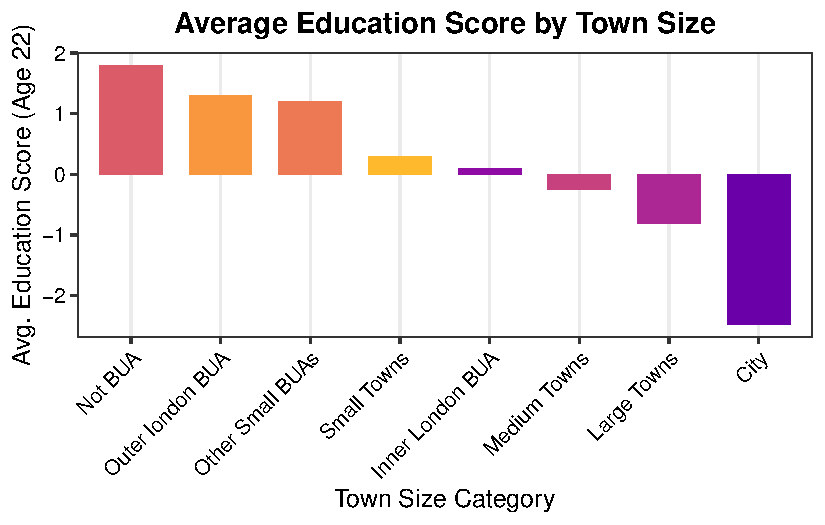
\includegraphics[keepaspectratio]{assignment3-paper_files/figure-pdf/fig-size-distribution-1.pdf}}

}

\caption{\label{fig-size-distribution}Average Education Score by Town
Size Category}

\end{figure}%

\subsection{Results}\label{results}

Figure~\ref{fig-map} shows the spatial distribution of education scores
across English towns. Higher scores tend to cluster in the East and
South East regions, particularly around Cambridge, Oxford, and the
commuter belt near London. In contrast, towns in the North and some
coastal regions report lower average education scores by age 22. This
geographic trend reflects broader regional disparities in post-secondary
educational outcomes.

We also explored which characteristics might predict full-time education
participation at age 19. While factors such as university presence,
income levels, and town size appeared relevant, further analysis was
limited by non-numeric data types and inconsistent indicator formats. As
such, we focused on mapping overall education performance, which more
reliably captured spatial patterns in town-level outcomes.

These results suggest that both regional context and access to
educational infrastructure play a role in shaping long-term academic
achievement. The map highlights specific areas where targeted investment
or policy support may improve educational trajectories.

\begin{figure}[H]

\centering{

\pandocbounded{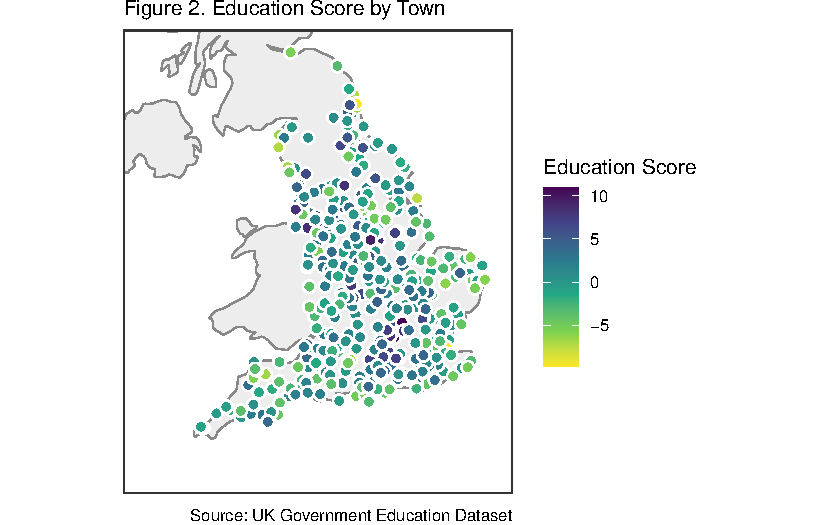
\includegraphics[keepaspectratio]{assignment3-paper_files/figure-pdf/fig-map-1.pdf}}

}

\caption{\label{fig-map}Education Score by Town}

\end{figure}%

\subsection{Discussion}\label{discussion}

The spatial analysis of education scores reveals notable regional
patterns across English towns. Higher scores are concentrated in the
South East, particularly near academic hubs such as Cambridge and
Oxford. These areas often benefit from stronger educational
infrastructure, greater economic resources, and proximity to
universities, which collectively support better post-secondary outcomes.

In contrast, towns in the North and along the coast display consistently
lower education scores. This disparity may reflect differences in access
to higher education, economic opportunities, or local investment in
youth development. Although the original aim included identifying
predictors of full-time higher education participation at age 19,
limitations in data format and variable types restricted deeper
statistical modelling. Nonetheless, the geographic distribution of
education outcomes remains clear and informative.

Interestingly, while it was expected that larger towns and cities would
outperform smaller ones, the analysis found that \emph{some smaller or
non-BUA areas had higher average education scores}, while \emph{cities
and large towns tended to lag}. This challenges assumptions about urban
advantage and suggests that education quality may not always scale with
town size. These findings raise further questions about local education
systems, cost of living, and community-level support structures.

\subsection{Conclusion}\label{conclusion}

The analysis highlights a strong connection between town characteristics
and educational attainment. Towns in economically advantaged or
university-adjacent regions are more likely to report higher average
education scores, while others---particularly in the North or on the
coast---tend to fall behind. Additionally, the lower scores seen in
cities and large towns indicate that educational outcomes are not solely
a function of urban access, but may also be influenced by local
pressures or resource disparities.

Despite some limitations, the results point toward meaningful spatial
trends that should inform future policy. Ensuring that young people,
regardless of where they live, have equal access to quality education
remains a critical goal.

\subsection{Recommendations}\label{recommendations}

\begin{itemize}
\tightlist
\item
  \textbf{Prioritise Investment in Underserved Regions:} Towns with
  consistently lower education scores---particularly in the North,
  coastal areas, and certain urban centers---should receive targeted
  funding and policy attention.
\item
  \textbf{Improve Data Consistency:} Future datasets should aim for
  clearer documentation and standardized variable formats to enable more
  robust modelling and comparative analysis.
\item
  \textbf{Expand Local Education Support:} Increasing access to higher
  education in smaller towns and underperforming urban areas through
  outreach, transport support, and scholarship programs could help
  address current gaps.
\item
  \textbf{Conduct Further Research:} Future studies could explore
  interactions between economic indicators, infrastructure quality, and
  education outcomes to build a more holistic understanding of regional
  disparities.
\end{itemize}

\subsection{References}\label{references}

This report used educational data sourced from the UK Office for
National Statistics (Office for National Statistics 2023), and town
coordinates were obtained using the \texttt{tidygeocoder} package
(Sadler 2023).

The following R packages were used throughout the analysis:

\begin{itemize}
\tightlist
\item
  \texttt{tidyverse} (Wickham 2023)
\item
  \texttt{dplyr} (Wickham et al. 2023)
\item
  \texttt{janitor} (Firke 2023)
\item
  \texttt{here} (Bryan, Hester, and Marwick 2023)
\item
  \texttt{kableExtra} (Dong 2023)
\item
  \texttt{tidygeocoder} (Sadler 2023)
\item
  \texttt{viridis} (Garnier 2023)
\item
  \texttt{R} (R Core Team 2024)
\end{itemize}

\phantomsection\label{refs}
\begin{CSLReferences}{1}{0}
\bibitem[\citeproctext]{ref-here}
Bryan, Jenny, Jim Hester, and Ben Marwick. 2023. \emph{Here: A Simpler
Way to Find Your Files}. \url{https://CRAN.R-project.org/package=here}.

\bibitem[\citeproctext]{ref-kableExtra}
Dong, Zhuoer. 2023. \emph{kableExtra: Construct Complex Table with
'Kable' and Pipe Syntax}.
\url{https://CRAN.R-project.org/package=kableExtra}.

\bibitem[\citeproctext]{ref-janitor}
Firke, Sam. 2023. \emph{Janitor: Simple Tools for Examining and Cleaning
Dirty Data}. \url{https://CRAN.R-project.org/package=janitor}.

\bibitem[\citeproctext]{ref-viridis}
Garnier, Simon. 2023. \emph{Viridis: Colorblind-Friendly Color Maps for
r}. \url{https://CRAN.R-project.org/package=viridis}.

\bibitem[\citeproctext]{ref-english_education_2024}
Office for National Statistics. 2023. {``Educational Attainment of Young
People in English Towns.''}
\url{https://www.ons.gov.uk/peoplepopulationandcommunity/educationandchildcare/articles/whydochildrenandyoungpeopleinsmallertownsdobetteracademicallythanthoseinlargertowns/2023-07-25}.

\bibitem[\citeproctext]{ref-R}
R Core Team. 2024. \emph{R: A Language and Environment for Statistical
Computing}. Vienna, Austria: R Foundation for Statistical Computing.
\url{https://www.R-project.org/}.

\bibitem[\citeproctext]{ref-tidygeocoder_coords}
Sadler, Jesse. 2023. {``Tidygeocoder: Geocoding Made Easy.''}
\url{https://cran.r-project.org/package=tidygeocoder}.

\bibitem[\citeproctext]{ref-tidyverse}
Wickham, Hadley. 2023. \emph{The Tidyverse: Easily Install and Load the
'Tidyverse'}. \url{https://CRAN.R-project.org/package=tidyverse}.

\bibitem[\citeproctext]{ref-dplyr}
Wickham, Hadley, Romain Francois, Lionel Henry, and Kirill Müller. 2023.
\emph{Dplyr: A Grammar of Data Manipulation}.
\url{https://CRAN.R-project.org/package=dplyr}.

\end{CSLReferences}




\end{document}
